\documentclass[conference, 10pt]{IEEEtran}
\IEEEoverridecommandlockouts
\usepackage{geometry}
 \geometry{
 a4paper,
 total={170mm,257mm},
 left=25mm,
 right=25mm,
 top=20mm,
 bottom=20mm,
 }
\usepackage{cite}
\usepackage{subfigure}
\usepackage{hyperref}
\usepackage{amsmath,amssymb,amsfonts}
\usepackage{algorithmic}
\usepackage{graphicx}
\usepackage{textcomp}
\usepackage{xcolor}
\usepackage{float}
\pagenumbering{arabic}
\pagestyle{plain}
\def\BibTeX{{\rm B\kern-.05em{\sc i\kern-.025em b}\kern-.08em
    T\kern-.1667em\lower.7ex\hbox{E}\kern-.125emX}}
    
\begin{document}

\title{The terahertz transistor, a brief overview.}

\author{
\IEEEauthorblockN{Jeffrey Gorissen}
\IEEEauthorblockA{\textit{Faculty of Industrial Engineering, Student number: 1436845}\\
jeffrey.gorissen@student.uhasselt.be}
}

\maketitle
\thispagestyle{plain}

\begin{abstract}
In the world of technology innovation is key. To keep up with more's law silicon-based transistors are starting to lack. More transistors on a given surface area are required to keep scaling up computational power. Researchers are now proposing graphene as the base material for transistors.  Graphene shows a huge potential that is backed by facts. Down to the atomic level, graphene possesses features that no other substance does. It is cheap, highly conductive and only one atom thick. Furthermore, research and experiments suggest that graphene-based computation is nearing.\\
\end{abstract}

\begin{IEEEkeywords}
Graphene, Silicon, Germanium, Transistor, Research
\end{IEEEkeywords}

\maketitle

\section{Introduction}

The crucial part of a silicon-graphene-germanium transistor is graphene. However, silicon and germanium are well-known elements in the fabrication of transistors. The germanium transistor debuted in 1947. It was developed by William Shockley, John Bardeen and Walter Brattain and was demonstrated at Bell Laboratories. The first silicon transistor also debuted at Bell Laboratories, this was early on in 1954. It was developed by Morris Tanenbaum. The commercial release of this transistor was later in the same year. It was produced by Texas Instruments who pushed the technology along with Bell Laboratories. \cite{phys} \cite{germaniumhistory} \cite{transistorhistory} \cite{losthistory}\\

Back to the present time, everybody is talking about graphene. When reading some of its basic properties, one might wonder if people were confusing it with a substance found in science fiction. Properties of graphene include that it is one atom thick, conducts electricity better than silicon, copper and even silver, conducts heat better than copper by a factor of ten, and it is stronger than steel by a factor of 200 while being six times lighter. \cite{graphene}\\


\section{Graphene}

Graphene is created from carbon, which only has two naturally occurring crystalline structures. The first, graphite, is just stacks and stacks of graphene piled on top of each other. The other, diamond, is a tetrahedral network of carbon atoms. These two natural states do not have a lot in common, except being built up from the same element, Carbon.\cite{graphene}\\

Diamond is an almost-perfect electrical insulator and graphite is a great conductor of heat and electricity. The arrangement of their atoms explains these differences. Carbon has four electrons on the valence shell. To form diamond each of those four electrons bond to carbon atoms around it. All of those tetrahedrons form a crystal structure. Due to this crystal structure, a diamond is extremely rigid and strong. This also explains why diamond is an insulator. There are no free electrons on the valence shell to carry a current.\cite{graphene}\\

On the other side, there is graphite. Each carbon atom in graphite is bonded to three other carbon atoms. These atoms align in such a manner that they form a sheet of hexagons. In this two-dimensional sheet, each atom has one free electron. These unpaired electrons are free to move when an electric current is applied. Now, graphite is a great conductor if you look at it in that two-dimensional sheet. However, in its natural state, it consists of layers of those sheets. This means that when a current is applied, the free electrons can move in, virtually, any direction. \cite{graphene}\\

This is where graphene turns up. If you strip away all those layers, eventually you end up with just a single layer, this single layer or sheet is called graphene. This can be seen in Figure \ref{fig:graphene}. The unpaired electrons are now only able to move in two directions, making graphene a fantastic electrical conductor. By not being molecularly bonded to each other, these sheets of carbon are rather easy to separate from one another. The layers are held together by Van Der Waal's bonds. This is a weak, electrostatic bond. \cite{graphene}

\begin{figure}[H]
\centering
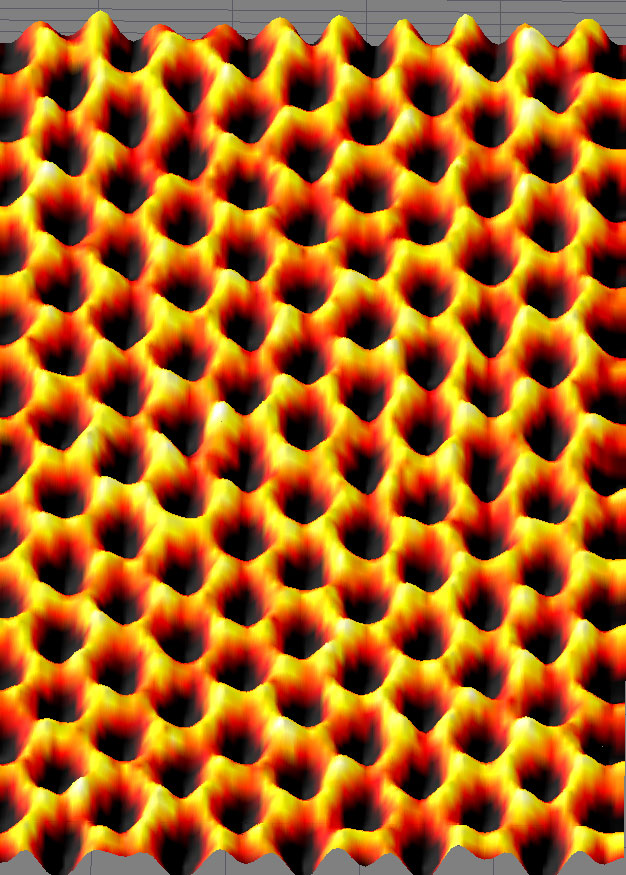
\includegraphics[width=0.25\textwidth, angle=90]{Img/graphene.jpg}
\caption{Scanning probe microscopy image of graphene. \cite{microscope}}
\label{fig:graphene}
\end{figure}

This is why the scientific community looking towards graphene as the replacement for silicon in microchips. Free electrons flow quicker across graphene. Meaning that an electron can move from one side of the graphene sheet to the other in a straight line without deviating around atomic imperfections. They think that graphene transistors could operate at frequencies that range into the Terra Hertz regions. This is about ten times the current maximum of silicon.\\

The biggest problem with graphene is the fabrication process. The process, at this moment, is not scaleable. It is possible to produce graphene in several different ways. Exfoliation, hydrothermal self-assembly, hydrothermal reduction, chemical vapour deposition, nanotube slicing, carbon dioxide reduction, spin coating, supersonic spray, microwave-assisted oxidation and ion implantation are some of the production methods currently known. The problem with the current techniques is that the graphene obtained from most of these processes is relatively low quality. The issue at hand is a purity problem. However, the silicon industry faced the same purity problems fifty years ago. Which gives this set-back hope. \cite{Production}\\

\section{Silicon-graphene-germanium transistor}
With everything in mind, it seems logical that a graphene-based transistor has the potential to increase the speed, and therefore, the performance of transistors. This is exactly what a team of researchers at the Institute of Metal Research, Chinese Academy of Sciences had in mind. They built the first transistor that works based on graphene. This was achieved by stacking an n-type top single-crystal Si membrane, a middle single-layer graphene, and an n-type bottom Ge substrate together. \cite{article1}\\

This Silicon-graphene-germanium transistor benefits from a Schottky emitter. The charging time of this emitter amounts to about 118 ps with the current being 692 A cm$^{-2}$ and value of 41 nF cm$^{-2}$ for the capacitance. Due to this, the researchers believe that the alpha cut-off frequency of the transistor can be increased from 1 MHz to well above 1 GHz. The expectation is that this can be realised going from using the previous tunnel emitters to using the current Schottky emitter.\cite{article1}\\

``With further engineering, the vertical semiconductor–graphene–semiconductor transistor is expected as one of the most promising devices for ultra-high-frequency operation in future 3D monolithic integration, because it combines the merits of the atomic thickness and high carrier mobility of graphene and the high feasibility of a Schottky emitter.'' \cite{article1}\\

Back in 2017, researchers at Northwestern University, Illinois started to investigate graphene-based logic gates. In their research, they describe the properties of graphene as "exceptional". In carbon-based logic, the current is the state variable. In conventional computing, voltage is the state variable. This leads to delays due to the limitation of charge transfer and accumulation in transistors. Therefore, graphene will make faster computation possible.\cite{article2}\\

"The exceptional material properties of carbon materials permit Terahertz operation and two orders of magnitude decrease in power-delay product compared to cutting-edge microprocessors. We hope to inspire the fabrication of these cascaded logic circuits to stimulate a transformative generation of energy-efficient computing." \cite{article2}\\

\section{Conclusion}
Presently, the graphene-based transistors are nowhere near the terahertz territory, yet. Luckily history puts this into a different perspective. Microprocessors in the early 1970s had frequencies ranging from a couple 100 kHz to 1 MHz (1973). In the past 10 years, speeds of over 5 GHz have been recorded for silicon-based consumer-grade microprocessors. \cite{Microprocessor}\\

A lot of research is going into the development of a commercial viable graphene-based transistor. The limits of silicon are forcing scientists to look elsewhere. The use of graphene will improve clock speeds, and decrease the energy needed to power microprocessors. Furthermore, this technology would enable smaller chips that fit even more transistors. All-carbon computing systems currently still do not exist. But the question is "when" rather then "if". With more research, this surely is the basis of the next-generation microprocessors.\\



\begin{thebibliography}{00}

\bibitem{phys} Chinese Academy of Sciences, 'Researchers build a silicon-graphene-germanium transistor for future THz operation', phys.org, 2019. [Online]. Available: \url{https://phys.org/news/2019-11-silicon-graphene-germanium-transistor-future-thz.html} [Accessed: 10-Nov-2019]

\bibitem{germaniumhistory} E. Darby, 'A History of Germanium', Van Heuvelen Lab, Unknown. [Online]. Available: \url{http://blogs.hmc.edu/vanheuvelen/the-elements/a-history-of-germanium-by-emily-darby/} [Accessed: 13-Nov-2019]

\bibitem{transistorhistory} T. Watkins, 'The History of the Transistor', San José State University, Unknown. [Online]. Available: \url{http://www.sjsu.edu/faculty/watkins/transist.htm} [Accessed: 15-Nov-2019]

\bibitem{losthistory} M. Riordan, 'The Lost History of the Transistor', IEEE Spectrum, 2004. [Online]. Available: \url{https://spectrum.ieee.org/tech-history/silicon-revolution/the-lost-history-of-the-transistor} [Accessed: 18-Nov-2019]

\bibitem{graphene}  M. Berger, 'What is graphene?', Nanowerk, 2019. [Online]. Available: \url{https://www.nanowerk.com/what_is_graphene.php} [Accessed: 18-Nov-2019]

\bibitem{microscope} U.S. Army Materiel Command, 'Graphene', 2012. [Online]. Available: \url{https://www.flickr.com/photos/armymaterielcommand/6795812766} [Accessed: 20-Nov-2019]

\bibitem{Production} L. Johnson, J. E. Meany, 'Mass-Producing Graphene', American Scientist, 2019. [Online]. Available: \url{https://www.americanscientist.org/article/mass-producing-graphene} [Accessed: 18-Nov-2018]

\bibitem{article1}  Liu, C., Ma, W., Chen, M. et al. A vertical silicon-graphene-germanium transistor. Nat Commun 10, 4873 (2019) doi:10.1038/s41467-019-12814-1 [Online]. Available: \url{https://www.nature.com/articles/s41467-019-12814-1} [Accessed: 20-Nov-2019]

\bibitem{article2} Friedman, J. S. et al. Cascaded spintronic logic with low-dimensional carbon. Nat. Commun. 8, 15635 doi: 10.1038/ncomms15635 (2017). [Online]. Available: \url{https://www.nature.com/articles/ncomms15635} [Accessed: 20-Nov-2019]

\bibitem{Microprocessor} Wikipedia, 'Microprocessor chronology', 2019. [Online]. Available: \url{https://en.wikipedia.org/wiki/Microprocessor_chronology} [Accessed: 26-Nov-2019]




\end{thebibliography}

\end{document}
